%
% $XORP: xorp/docs/design_arch/design_arch.tex,v 1.23 2006/08/02 00:29:09 pavlin Exp $
%

\documentclass[11pt]{article}

%\usepackage[dvips]{changebar}

\usepackage{subfigure}
\usepackage{fullpage}
\usepackage{setspace}
\usepackage{times}
\usepackage{latexsym}
\usepackage{epsfig}
\usepackage{graphicx}
\usepackage{xspace}
\usepackage{color}
\usepackage{amsmath}
\usepackage{rotating}
\usepackage{moreverb}
\usepackage{listings}
\usepackage{alltt}
\usepackage{stmaryrd}
%\usepackage[dvipdf]{graphics}
%\usepackage[dvips]{graphicx}
%\usepackage{xorp}

\definecolor{gray}{rgb}{0.5,0.5,0.5}
\newcommand{\etc}{\emph{etc.}\xspace}
\newcommand{\ie}{\emph{i.e.,}\xspace}
\newcommand{\eg}{\emph{e.g.,}\xspace}
%\newcommand{\comment}[1]{{\color{gray}[\textsf{#1}]}}
%\newcommand{\comment}[1]{}

% Changebar stuff
% \newenvironment{colorcode}{\color{blue}}{}
% \renewcommand{\cbstart}{\begin{colorcode}}
% \renewcommand{\cbend}{\end{colorcode}}

% \pagestyle{empty}

\begin{document}

\title{XORP Design Overview \\
\vspace{1ex}
Version 1.3}
\author{ XORP Project					\\
	 International Computer Science Institute	\\
	 Berkeley, CA 94704, USA			\\
         {\it http://www.xorp.org/}			\\
	 {\it feedback@xorp.org}
}
\date{August 2, 2006}

\maketitle


%%%%%%%%%%%%%%%%%%%%%%%%%%%%%%%%%%%%%%%%%%%%%%%%%%%%%%%%%%%%%%%%%%%%%%%
\section{Introduction}

This document provides a brief overview of the XORP (eXtensible Open
Router Platform) architecture. It is intended both for people who are
interested in the architecture itself, and as a starting point for developers
who wish to modify the software.  People who are interested in the XORP
multicast routing architecture should read also
\cite{xorp:multicast_arch}.

%%%%%%%%%%%%%%%%%%%%%%%%%%%%%%%%%%%%%%%%%%%
\subsection{XORP Motivation}

A gap exists between network research and Internet practice due to the
nature of the Internet router software business.  It is really hard
for researchers to introduce new protocols and mechanisms into
operational networks, and to study existing protocols in the wild.
The primary goal of XORP is to fill this gap.  To succeed it must be both
a research tool and a stable deployment platform that can be used in
production networks.  It must also place a strong emphasis on
extensibility, while coping with the impact of this on robustness,
security and performance.

For more details about the XORP design {\it philosophy}, see
\cite{handley:hotnets2002:xorp}.

%%%%%%%%%%%%%%%%%%%%%%%%%%%%%%%%%%%%%%%%%%%%%%%%%%%%%%%%%%%%%%%%%%%%%%%
\section{Target}

The goal for XORP is to become a suitable software platform that can
be used as the core of practically any router. However, the {\it
initial} focus is on an edge router running on commodity PC hardware
with relatively low port density and moderate size routing
tables~\footnote{A comparable production router might be a Cisco
7206VXR (or pretty much anything smaller than this).}.

However, given the flexibility of the XORP architecture, in the future
we should not be limited to edge-router scenarios or PC hardware.  For
example:
\begin{itemize}

  \item We can easily imagine using multiple PCs as forwarding engines,
  with a single control element. This would allow greater port density.

  \item Another useful target would be a PC with a number of network
  processors (\eg Intel IXP1200) doing the bulk of the forwarding.

  \item Finally, in the long run, the code base might be run the
  control processor of high-performance ASIC-based routers.

\end{itemize}

%%%%%%%%%%%%%%%%%%%%%%%%%%%%%%%%%%%%%%%%%%%%%%%%%%%%%%%%%%%%%%%%%%%%%%%
\section{Functionality}

XORP is designed to support both IPv4 and IPv6.
Below is our initial target list of protocols and features to be
supported by XORP. Those in bold are already implemented or supported
to some degree. Not all of the implemented features have been tested
yet.

%%%%%%%%%%%%%%%%%%%%%
\subsubsection*{Unicast Routing Protocols}

\begin{itemize}
  \item {\bf BGP4+} ({\bf IPv4} and {\bf IPv6})
  \item {\bf OSPF} ({\bf IPv4} and IPv6)
  \item {\bf RIPv2 (IPv4)}, {\bf RIPng (IPv6)}
  \item IS-IS
\end{itemize}

%%%%%%%%%%%%%%%%%%%%%
\subsubsection*{Multicast Routing Protocols}

\begin{itemize}
  \item {\bf PIM-SM, PIM-SSM}, Bidir-PIM ({\bf IPv4} and {\bf IPv6})
  \item {\bf IGMPv1, v2, v3} ({\bf IPv4})
  \item {\bf MLDv1, v2} ({\bf IPv6})
\end{itemize}

%%%%%%%%%%%%%%%%%%%%%
\subsubsection*{Network Management}

\begin{itemize}
  \item {\bf Command Line Interface} (similar to Juniper)
  \item {\bf SNMP}
  \item WWW
\end{itemize}

%%%%%%%%%%%%%%%%%%%%%
\subsubsection*{Forwarding Path}

\begin{itemize}
  \item {\bf Traditional UNIX forwarding path}
  \item {\bf Click forwarding path}
  \item {\bf Windows Server 2003 forwarding path}
  \item User-level simulation-like environment
\end{itemize}

%%%%%%%%%%%%%%%%%%%%%
\subsubsection*{Miscellaneous}

\begin{itemize}
  \item {\bf Routing policies} ({\bf unicast} and multicast)
\end{itemize}

%%%%%%%%%%%%%%%%%%%%%%%%%%%%%%%%%%%%%%%%%%%%%%%%%%%%%%%%%%%%%%%%%%%%%%%
\section{Architecture}

%%%%%%%%%%%%%%%%%%%%%%%%%%%%%%%%%%%%%%%%%%%
\subsection{Design Philosophy}

The XORP design philosophy stresses {\em extensibility},
{\em performance} and {\em robustness}.

For routing and management modules, the primary goals are
extensibility and robustness.  These goals are achieved by carefully
separating functionality into independent modules, running in separate
UNIX processes, with well-defined APIs between them.  Clearly, there
are performance penalties to pay for such an architecture, but we
believe that so long as careful attention is paid to computational
complexity, the costs associated with inter-process communication will
be acceptable given the obvious extensibility and robustness benefits.

For the forwarding path, the primary goals are extensibility and
performance.  Robustness here is primarily achieved through
simplicity and a modular design that encourages re-use of well-tested
components.


%%%%%%%%%%%%%%%%%%%%%%%%%%%%%%%%%%%%%%%%%%%
\subsection{Design Overview}

XORP can be divided into two subsystems. The higher-level
(``user-space'') subsystem consists of the routing protocols and
management mechanisms. The lower-level (``kernel'') provides the
forwarding path, and provides APIs for the higher-level to access.

User-level XORP uses a multi-process architecture with one process per
routing protocol, and a novel inter-process communication mechanism
known as XORP Resource Locators (XRLs)~\cite{xorp:xrl}. XRL
communication is not limited to a single host, and so XORP can in
principle run in a distributed fashion. For example, we can have a
distributed router, with the forwarding engine running on one machine,
and each of the routing protocols that update that forwarding engine
running on a separate control processor system.

The lower-level subsystem can use traditional UNIX kernel forwarding,
the Click modular router~\cite{CLICK-PROJECT} or Windows kernel
forwarding (Windows Server 2003). The modularity and minimal
dependencies between the lower-level and user-level subsystems allow for
many future possibilities for forwarding engines.  As standards such as
those being developed in the IETF ForCES Working Group emerge, we expect
to support them to provide true forwarding engine interchangeability.

\begin{figure}[htbp]
  \begin{center}
    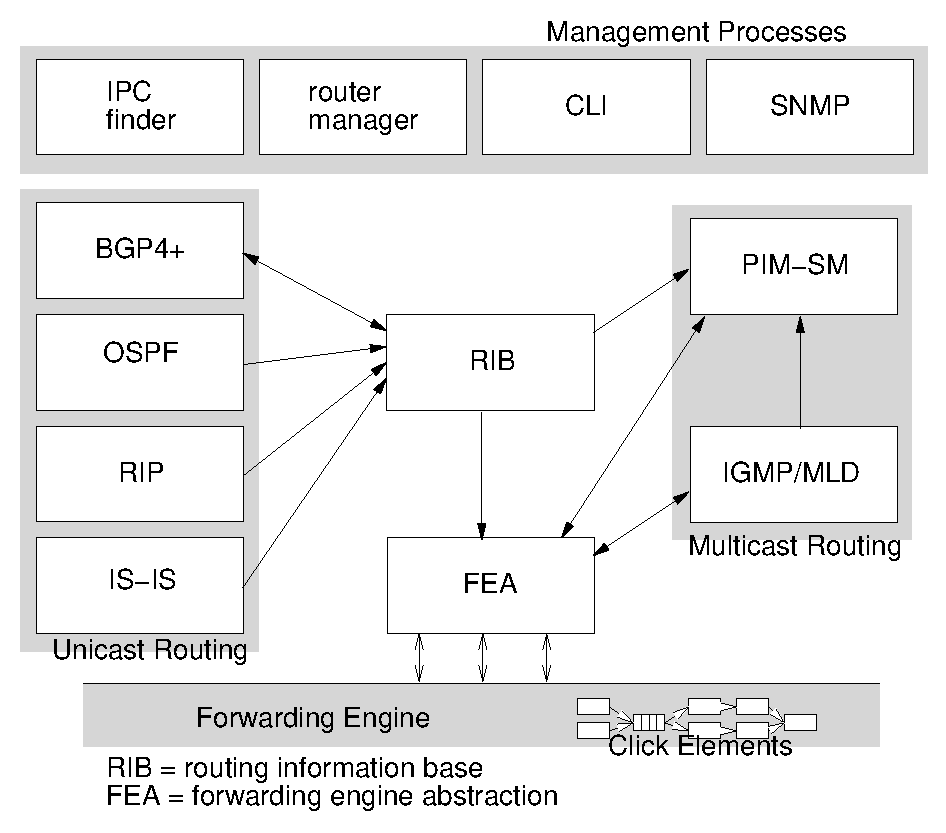
\includegraphics[width=0.7\textwidth]{figs/processes3.ps}
    % \vspace{.05in}
    \caption{XORP Process Model}
    \label{fig:process_model}
  \end{center}
\end{figure}

Figure~\ref{fig:process_model} shows the processes in XORP, although
it should be noted that some of these modules use separate processes
to handle IPv4 and IPv6. For simplicity, the arrows show only the
main communication flows used for routing information.  Control flows
are not shown - for example, the FEA may need to inform the routing
processes when an interface goes down. These processes are further
described in Section~\ref{sec:xorp_processes_description}.

We should note that even though our design philosophy is that each
XORP component in Figure~\ref{fig:process_model} will run as a
separate process, it would also be possible to compile most of them
together to run as one single process. Obviously, the robustness of
such a router would suffer because the crash of a single component
would bring down the whole router. However, the XORP architecture is
designed to be flexible, and other developers building on this
software can choose to use it in different ways.

%%%%%%%%%%%%%%%%%%%%%%%%%%%%%%%%%%%%%%%%%%%
\subsection{XORP Processes Description}
\label{sec:xorp_processes_description}

%%%%%%%%%%%%%%%%%%%%%
\subsubsection{FEA (Forwarding Engine Abstraction)}

The FEA provides a platform independent interface to the basic routing
and network interface management functionality.
For example, get or set information about network interfaces, install or
modify unicast forwarding entries, multicast routing support, etc.

If the router is distributed, in the sense that some
Forwarding Engines (FEs) are not in the same chassis as the control
software, then the FEA will also handle control communications with the
remote FEs.  Note that, strictly speaking, it is not required that all
communication with the FE must go through the FEA. For example, Click
modules can communicate directly with a user-space process. However,
the FEA abstracts all the details about the underlying system
from the user-level XORP processes; therefore by using the common API
provided by the FEA we can greatly simplify the rest of the XORP
components.

Note that the multicast-related functionalities are logically separated from
the unicast-based functionalities in the MFEA (Multicast Forwarding Engine
Abstraction), though the MFEA is part of the FEA process.

For more information about the FEA see \cite{xorp:fea}.
For more information about the MFEA see \cite{xorp:mfea}.

%%%%%%%%%%%%%%%%%%%%%
\subsubsection{RIB (Routing Information Base)}

The RIB holds a user-space copy of the entire routing/forwarding table,
complete with information about where each route came from (\eg which
protocol, and when). It communicates with the routing protocols such as
BGP, RIP and OSPF to instantiate routes, and with the FEA to install the
appropriate forwarding entries in the FEs.

The RIB also holds the routing information for multicast-capable routes
(MRIB) to be used for multicast Reverse-Path Forwarding (RPF) information.
For example, PIM-SM uses the MRIB information to route joins/prunes and
to determine the RPF interface for sources and for RPs.

The MRIB is populated by whatever ``unicast'' protocol is used to
provide multicast capable path information. Typically this is
MBGP for inter-domain paths, where it is possible to tell the
difference between unicast-capable and multicast-capable routers.  For
intra-domain routing, this usually is the regular unicast FIB
information.

Note that for unicast, routing and forwarding tables are practically the
same. In case of multicast, the RIB provides the RPF information, while
the forwarding information (the incoming and outgoing interfaces) is
computed by the particular multicast routing protocol. The multicast
forwarding information is kept by the multicast routing protocol itself, and
installed directly through the FEA. In the future, when there is more
than one multicast routing protocols, XORP may have the multicast
equivalent of RIB that would be responsible for coordinating among the
different multicast routing protocols running on the same router.

On a router with multiple FEs, the RIB is responsible for splitting
up the routing table amongst the FEs and for figuring out how to forward
between FEs.

For more information about the RIB see \cite{xorp:rib}.

%%%%%%%%%%%%%%%%%%%%%
\subsubsection{BGP4+}

This is the BGP routing daemon. It implements IPv4 and IPv6 unicast
routing in a single process, as well as MBGP for both IPv4 and IPv6
multicast RIBs for multicast routing purpose.

For more information about the XORP BGP implementation, see \cite{xorp:bgp}.

%%%%%%%%%%%%%%%%%%%%%
\subsubsection{OSPF}

This is the OSPF routing daemon. There are separate IPv4 and IPv6
daemons, because unlike BGP there is no real need to tie them together.

%%%%%%%%%%%%%%%%%%%%%
\subsubsection{RIP}

This is the RIP routing daemon. Similarly to OSPF, the IPv4 and IPv6
daemons are separate.

%%%%%%%%%%%%%%%%%%%%%
\subsubsection{MLD/IGMP}

This is Multicast Listener Discovery/Internet Group Management Protocol
handler. It implements the router-side part of MLD and IGMP. Its main
purpose is to discover local multicast members and propagate this
information to multicast routing daemons such as PIM-SM.
Similar to OSPF and RIP, the IGMP (IPv4) and MLD (IPv6) daemons are
separate.

For more information about the XORP MLD/IGMP implementation see
\cite{xorp:mld_igmp}.

%%%%%%%%%%%%%%%%%%%%%
\subsubsection{PIM-SM}

This is the PIM-SM multicast routing daemon. Similar to OSPF and RIP,
the PIM-SM IPv4 and IPv6 daemons are separate. The PIM-SM protocol requires
information about local multicast members, and Reverse-Path Forwarding
to operate properly. The former is obtained from the IGMP/MLD process;
the latter is obtained from the RIB.

For more information about the XORP PIM-SM implementation see
\cite{xorp:pim}.

%%%%%%%%%%%%%%%%%%%%%
\subsubsection{RTRMGR: XORP Router Manager}

The {\em rtrmgr} is the process responsible for starting all components of
the router, to configure each of them, and to monitor and restart any
failing process.  It also provides the interface for the CLI to change
the router configuration.

For more information about the {\em rtrmgr} see
\cite{xorp:rtrmgr}.

%%%%%%%%%%%%%%%%%%%%%
\subsubsection{CLI: Command Line Interface}

The CLI can be used by an user to access the router, view
its internal state, or to configure it on-the-fly. Its functionality
is closely related to the {\em rtrmgr}. However, because the robustness of
the {\em rtrmgr} itself is extremely important, all functionality that can
be run as a separate CLI process are separated from the {\em rtrmgr}.  The
process implementing this CLI functionality is called {\em xorpsh}.

For more information about the CLI and the xorpsh process see
\cite{xorp:rtrmgr}.

%%%%%%%%%%%%%%%%%%%%%
\subsubsection{Inter-Process Communication Finder}

The IPC finder is needed by the communication method used among all
XORP components, \ie the XRLs. Each of the XORP components registers
with the IPC finder. The finder assists the XRL communications (more
specifically, it knows the location of each XRL target), therefore a
XORP process does not need to know explicitly the location of all
other processes, or how to communicate with them.  The router manager
process ({\em rtrmgr}) incorporates a finder, so a separate finder process
is only needed if the {\em rtrmgr} is not being used such as during testing.

For more information about the IPC finder and XRLs see
\cite{xorp:xrl} and \cite{xorp:xrl_interfaces}.

%%%%%%%%%%%%%%%%%%%%%
\subsubsection{SNMP}

This is the SNMP management process. It is used for SNMP access to the
router. For example, it can be used to translate SNMP requests into XRL
requests. Internally, SNMP will communicate with the other processes
using XRLs.

%%%%%%%%%%%%%%%%%%%%%
\subsubsection{Routing Policies}

This is the routing policies coordination process.~\footnote{This
process is not shown in Figure~\ref{fig:process_model} for simplicity
purpose.} It interacts with all routing protocols and RIB and instructs
them how the handle the routes flowing to the system: export routes from
one protocol to another, modify or remove routes as they flow through
the system, etc.  Currently only unicast routing policies are supported.

%%%%%%%%%%%%%%%%%%%%%%%%%%%%%%%%%%%%%%%%%%%%%%%%%%%%%%%%%%%%%%%%%%%%%%%
%     APPENDIX
%%%%%%%%%%%%%%%%%%%%%%%%%%%%%%%%%%%%%%%%%%%%%%%%%%%%%%%%%%%%%%%%%%%%%%%
\appendix
\section{Modification History}

\begin{itemize}

  \item December 11, 2002: Initial version 0.1 completed.

  \item March 10, 2003: Updated to match XORP release 0.2.

  \item June 9, 2003: Updated to match XORP release 0.3.

  \item August 28, 2003: Updated to match XORP release 0.4: SNMP
  is implemented.

  \item November 6, 2003: Updated to match XORP release 0.5: BGP
  supports IPv6.

  \item July 8, 2004: Updated to match XORP release 1.0: RIP and RIPng
  are implemented.

  \item April 13, 2005: Updated to match XORP release 1.1: there is
  support for Click forwarding path.

  \item March 8, 2006: Updated to match XORP release 1.2: OSPF is
  implemented, there is policy support, and support for Windows
  forwarding path.

  \item August 2, 2006: Updated to match XORP release 1.3: IGMPv3 and
  MLDv2 are implemented.

\end{itemize}

%%%%%%%%%%%%%%%%%%%%%%%%%%%%%%%%%%%%%%%%%%%%%%%%%%%%%%%%%%%%%%%%%%%%%%%
%     BIBLIOGRAPHY
%%%%%%%%%%%%%%%%%%%%%%%%%%%%%%%%%%%%%%%%%%%%%%%%%%%%%%%%%%%%%%%%%%%%%%%
\bibliography{../tex/xorp}
\bibliographystyle{plain}

%%%%%%%%%%%%%%%%%%%%%%%%%%%%%%%%%%%%%%%%%%%%%%%%%%%%%%%%%%%%%%%%%%%%%%%
\end{document}
